\chapter{FISSA - Fault Injection Simulation for Security Assessment}
\chaptermark{FISSA - Fault Injection Simulation for Security Assessment}
\label{chapter:fissa}
\minitoc

This section introduces and presents a tool, called FISSA -- Fault Injection Simulation for Security Assessment --, created to automate fault injection attacks campaigns in simulation. The first section will presents the state of the art of existing tools for FIA campaigns in emulation, formal methods or even perform real world attacks. The second section will presents the architecture and details how FISSA works and presents how to extend it depending on other needs. Finally, I will discuss about it and draw some perspectives for the tool's development and usability.

%%%%%%%%%%%%%%%%%%%%%%%%%%%%%%%%%%%%%%%%%%%%%%%%%%%%%%%%%%%%%%%%%%%%%%%%%%%%%%%%%%%%%%%%%%%%%%%
\section{Simulation tools for Fault Injection}
This section presents recent works related to methods and tools for vulnerability assessment when considering fault injection attacks. For such vulnerability assessment, main strategies include actual fault injections, emulations, formal methods and simulations.

\begin{table}[t]
    \centering
    \caption{Fault Injection based methods for vulnerability assessment comparison}
    \label{table:FI_type_comparison}
    \normalsize
    \setlength{\tabcolsep}{1pt}
    \begin{tabular}{@{}lccccccc@{}}
        \toprule
                          & References  & Cost                                & \begin{tabular}[c]{@{}c@{}}Control over\\fault scenarios\end{tabular}       & Scalability                         & Speed of execution                                      & Realism                             & Expertise \\ \midrule
        Formal Methods    & \cite{BSSMG-21-tchess, ANR-18-ices, BBCFGS-19-esorics, SVPMRDKMS-24-eprint}     & \textcolor{ForestGreen}{Very low}  & \textcolor{ForestGreen}{Very high}  & \textcolor{red}{Very low}           & \textcolor{red}{Low}                                    & \textcolor{red}{Low}                & \textcolor{red}{Very high} \\
        Simulations  & \cite{AB-23-acns, fisim, AWMN-20-host}     & \textcolor{ForestGreen}{Very low}       & \textcolor{ForestGreen}{Very high}  & \textcolor{red}{Low}                & \textcolor{red}{Low}/\textcolor{ForestGreen}{Moderate}  & \textcolor{ForestGreen}{Moderate}   & \textcolor{ForestGreen}{Low} \\
        Emulations        & \cite{CMLCVR-11-crypto, HGASO-21-fdtc,BLK-23-access, NNHRS-14-dsd}     & \textcolor{Red}{High}           & \textcolor{ForestGreen}{Moderate}   & \textcolor{ForestGreen}{High}  & \textcolor{ForestGreen}{Very high}                      & \textcolor{ForestGreen}{High}       & \textcolor{red}{Moderate} \\
        Actual FIA        & \cite{BCNTW-06-procieee, BFP-19-tches, GBD-23-paine, CGVCBLC-22-cardis}     & \textcolor{Red}{Very high}           & \textcolor{Red}{Very low}           & \textcolor{ForestGreen}{Very high}  & \textcolor{ForestGreen}{Very high}                      & \textcolor{ForestGreen}{Very high}  & \textcolor{red}{Very high} \\
        \bottomrule
    \end{tabular}
\end{table}

Actual FIAs involve physically injecting faults into the target hardware using techniques such as variations in supply voltage or clock signal~\cite{BCNTW-06-procieee, BFP-19-tches}, laser pulses~\cite{BCNTW-06-procieee, CGVCBLC-22-cardis}, electromagnetic emanations~\cite{BCNTW-06-procieee} or X-rays~\cite{GBD-23-paine}.
This approach offers valuable insights into the real impact of faults on hardware components.
However, a significant drawback of actual fault injections is that they demand considerable expertise to prepare the target, involving intricate setup procedures.
Additionally, this approach can only be executed once the physical circuit is available, potentially delaying the vulnerability assessment process until later stages of development.


Fault emulation can, for instance, rely on FPGA~\cite{CMLCVR-11-crypto}, or on an emulator such as QEMU~\cite{HGASO-21-fdtc,BLK-23-access} to perform fault injection campaigns. This approach is four times faster than simulation-based techniques~\cite{NNHRS-14-dsd}, and unlike simulation-based or formal method-based fault injections techniques, the size of the evaluated circuit has no major impact on the fault injection campaign timing performances.
However, configuring an emulation environment can be complex and time-consuming. Achieving an accurate representation of the target system may require detailed configuration and parameter tuning. The accuracy of emulation is contingent on the quality of the models used to replicate the target hardware. If the models are inaccurate or incomplete, the results of fault injections may not precisely reflect actual behaviour.

Formal methods provide an advantage with mathematical proofs, ensuring a rigorous verification of the system's behaviour during fault injection experiments. Formal methods approaches such as~\cite{BSSMG-21-tchess} allow the analysis of a circuit design in order to detect sensitive logic or sequential hardware elements. \cite{ANR-18-ices}, \cite{BBCFGS-19-esorics} and~\cite{SVPMRDKMS-24-eprint} present formal verification methods to analyse the behaviour of HDL implementation.
However, this type of tool usually suffers from restrictions limiting its actual usage on a complete processor.
Conventional formal approaches encounter scalability challenges due to limitations in verification techniques.
In particular, the circuit structure it can analyse is usually limited.

Fault Injections simulations can be performed at processor instructions level. Authors of~\cite{AB-23-acns} explore the impact of fault injection attacks on software security. They evaluate four open-source fault simulators, comparing their techniques and suggest enhancing them with AI methods inspired by advances in cryptographic fault simulation. \cite{fisim} is an open-source deterministic fault attack simulator prototype utilising the Unicorn Framework and Capstone disassembler.
\cite{AWMN-20-host} introduces VerFI, a gate-level granularity fault simulator for hardware implementations. For instance, it has been used to spot an implementation mistake in ParTI~\cite{SMG-16-crypto}.
However, this tool has been developed to check if implemented countermeasures can really protect against fault injection on cryptographic implementations, but it cannot evaluate components such as registers or memories.
In this paper, we focus on Cycle Accurate Bit Accurate (CABA) Simulation, which provides a controlled virtual environment for injecting faults. There are several solutions of simulations in an HDL simulator like Questasim, Vivado, etc. \textit{Behavioural} simulation is used to detect functional issues and ensuring that the design behaves as expected. \textit{Post-synthesis} simulation verifies that the synthesised netlist matches the expected functionality. \textit{Timed} simulation is used to ensure that the design meets timing requirements and can operate at the specified clock frequency. And finally, \textit{post-implementation} simulations are used to verify that the implemented design meets all requirements and constraints, including those related to the physical layout on the target.
Simulation-based fault injection offers the advantage of enabling designers to test their system throughout the design cycle, providing valuable insights and uncovering potential vulnerabilities early in the development process. However, a limitation lies in the potential lack of absolute fidelity to actual conditions, as simulations might not perfectly replicate all hardware intricacies, introducing a slight risk of overlooking certain faults that could manifest in the actual hardware.

Table~\ref{table:FI_type_comparison} shows a comparison between these four methods for vulnerability assessment when considering FIA regarding six metrics. These metrics are the financial cost of setting up the fault injection campaign, the control over fault scenarios (how configurable are the scenarios), scalability which refers to the method capacity to be applied to systems of different sizes or complexities, speed of execution of the campaign, realism of the fault injection campaign and the level of required expertise.
Table~\ref{table:FI_type_comparison} shows that no method is completely optimal. Each method has its own advantages and disadvantages and must be chosen by the designer according to the requirements and the available financial and human resources. Indeed, setting up an actual fault injection campaign requires much more expertise in this domain and also requires costly equipment, whereas setting up a simulation campaign can be easier for a circuit designer familiar with HDL simulation tools such as Questasim.
Table~\ref{table:FI_type_comparison} shows that CABA simulation offers a good compromise to assess the security level of a circuit design. In particular, it provides an efficient solution for investigating security throughout the design cycle, enabling the concept of “Security by Design”.

%%%%%%%%%%%%%%%%%%%%%%%%%%%%%%%%%%%%%%%%%%%%%%%%%%%%%%%%%%%%%%%%%%%%%%%%%%%%%%%%%%%%%%%%%%%%%%%
\section{FISSA}
\subsection{Main software architecture}

\begin{figure}[ht]
    \centering
    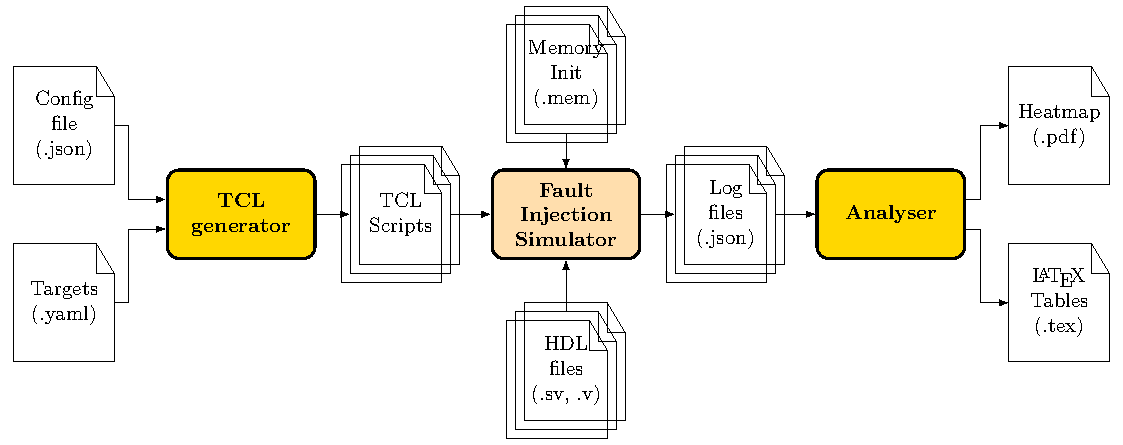
\includegraphics[width=\textwidth]{c4_fissa/img/fissa/archi_gen_tcl.pdf}
    \caption{Software architecture of FISSA}
    \label{fig:archi_fissa}
\end{figure}

\subsection{Supported fault models}

\subsection{TCL Generator}

\begin{figure}[ht]
    \centering
    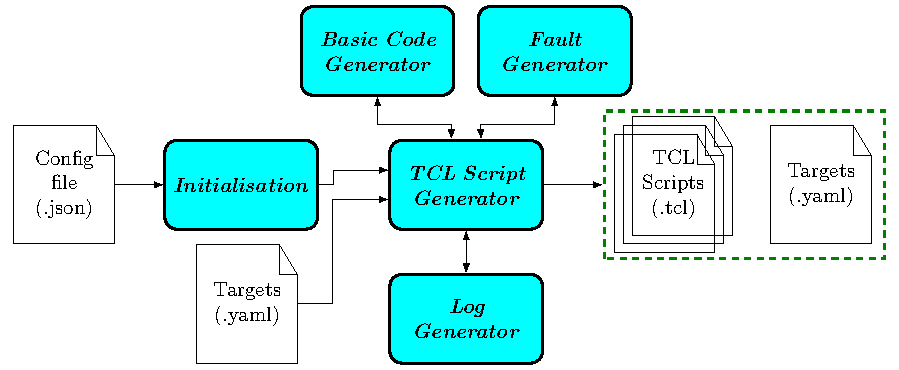
\includegraphics[width=\textwidth]{c4_fissa/img/fissa/detail_tcl_gen.pdf}
    \caption{Software architecture of the TCL Generator module}
    \label{fig:archi_tcl_gen}
\end{figure}

\subsection{Fault Injection Simulator}

\subsection{Analyser}

\subsection{Extending FISSA}

%%%%%%%%%%%%%%%%%%%%%%%%%%%%%%%%%%%%%%%%%%%%%%%%%%%%%%%%%%%%%%%%%%%%%%%%%%%%%%%%%%%%%%%%%%%%%%%
\section{Discussion and Perspectives}

%%%%%%%%%%%%%%%%%%%%%%%%%%%%%%%%%%%%%%%%%%%%%%%%%%%%%%%%%%%%%%%%%%%%%%%%%%%%%%%%%%%%%%%%%%%%%%%
\section{Summary}

%%%%%%%%%%%%%%%%%%%%%%%%%%%%%%%%%%%%%%%%%%%%%%%%%%%%%%%%%%%%%%%%%%%%%%%%%%%%%%%%%%%%%%%%%%%%%%%